\documentclass[a4paper, 12pt]{article}

% Packages
\usepackage{graphicx}
\usepackage[utf8]{inputenc}
\usepackage[backend=biber]{biblatex}
\usepackage{ifxetex}

% TUB Font
\ifxetex
   % Muli font
   \usepackage{xltxtra}
   \setmainfont{Muli}
\else
   % Arial font
   \usepackage{times}
   \renewcommand{\rmdefault}{\sfdefault}
\fi
\linespread{1.2}

% Settings
\graphicspath{ {images/} }
\addbibresource{bibliography.bib}

% Variables
\newcommand{\thesistitle}{model2regex: Detecting DGAs with Regular Expressions Generated by a Language Model}
\newcommand{\thesisauthor}{Eric Schneider}
\newcommand{\matrno}{365800}
\newcommand{\supervisor}{Alexander \textsc{Warnecke}, Tammo \textsc{Kr\"uger}}

\begin{document}

\begin{titlepage}
	\centering
	
\includegraphics[width=5cm]{tub-logo}\par\vspace{0.5cm}
	{Technische Universität Berlin \par}
	\vspace{2cm}
	{\large \textsc{Exposé}\par}
	\vspace{1cm}
	{\Large\bfseries \thesistitle\par}
	\vspace{2cm}
	%\vfill
	{\large \thesisauthor\par}
	{\large Matr. No. \matrno\par}
	\vspace{2cm}
	
\includegraphics[width=5cm]{mlsec-logo-red2}\par\vspace{0.5cm}
	{Chair of Machine Learning and Security \par}
	{Prof. Dr. Konrad Rieck \par}
	\vfill
	supervised by\par
	\supervisor
	\vfill
	\today\par
\end{titlepage}

\section{Introduction}
%Some intro to the topic: What is it about? What is the specific problem that should be addressed in this work?
Domain Generating Algorithms (DGAs) are increasingly used in botnets as part of
command and control (C\&C) communication. Malware creators use these algorithms
to generate multiple possible domains each day and then have their malware
contact a small portion of them to obfuscate the real server they are getting
their instructions and updates from. This tactic gives the attacker a huge
advantage, because to protect against it, means taking control of possible thousands
of domains, while the attacker only needs to control a short lived domain
executing their attack. Better protection may come from blocking
botnets at the source by recognizing communication with specific domains as
fraudulent or rather generated by a specific DGA family. DGAs however are
generated randomly and use different seeds from either specific dates, twitter
trends, hashes or word lists. Therefore static blocklists may not be able to
keep up with blocking the communication at a network level. Deep Learning
approaches have shown great promises and are currently state of the art in
detecting Algorithmically-Generated Domains (AGD). 
Machine learned models can be used to filter network traffic, setting them up for a filter pipeline
may not be very simple and also can be a black box on determining what exactly the model is
filtering.
Using algorithms from the field of language processing this thesis will attempt to learn the
structure of different DGA families trying to learn their structure and using that information to
generate regular expressions (RegEx). Resulting in an ease in implementing filters in existing
security architecture and showing a more human readable result to help understanding the structure
of learned DGAs.

\section{Methodology}
%What methodology will be applied in this work? That is, what is the general strategy to solve the
%problem this work is concearned with?
The main methodology of this thesis will be applied research. Using currently established solutions
from the field of language processing. The approach will be an iterative process of discovering
which approaches will be the most successful. Working with a prototype which is built as a classic
machine learning model, specifically a Gated Recurrent Unit (GRU) to learn the structure of a DGA
and then use the information of the hidden layers and the output to build a regular expression that
will represent the structure found by the language model. The main research will focus on exploring
methods and the possibility of extracting a regular expression out of the specialized model. 

\section{Approach}
%How is the implementation of the strategy approached?
As mentioned before I will iteratively explore the possibilities of turning a learned model into a
regular expression, so the beginning of the research will be working around exploring these
possibilities and iterating on implementations. Currently a small prototype exists that can learn
the banjori algorithm very reliably. 
The language model will have the following architecture:\\
\begin{figure}[h]
    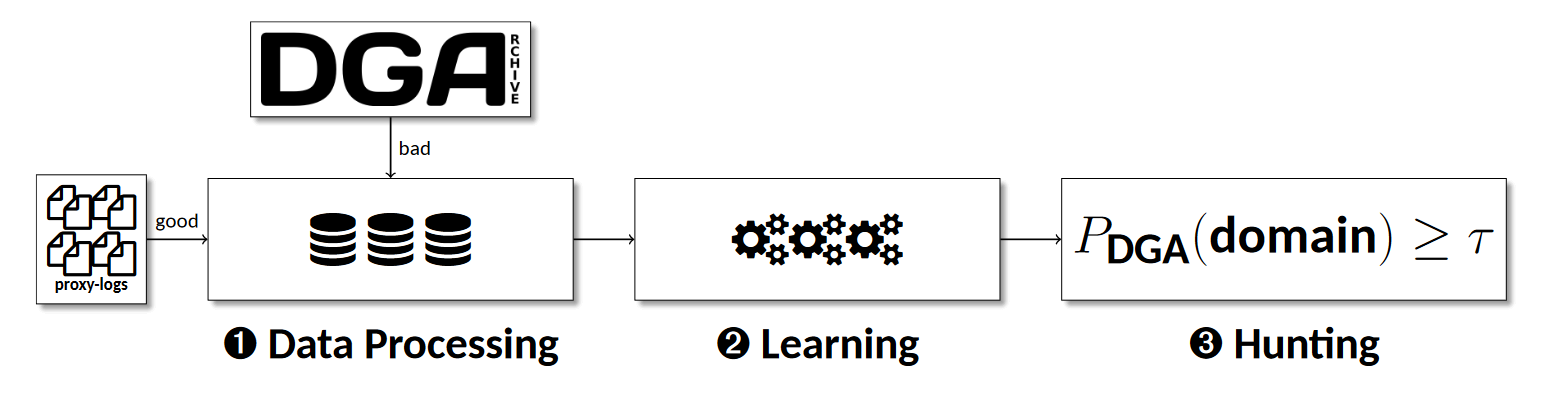
\includegraphics[width=\textwidth]{images/DGA_Detect_Architecture.png}
    \caption{Graphic provided by Tammo Kr\"uger}
\end{figure}\\
The learning part is already solved and does work with a decent accuracy, the last step (3) Hunting
is now what the main focus of the thesis will be. The majority of these 6 months I will work on this
part and at least 2 months will be used for setting up the evaluation described and on writing down
my results into the thesis.
\section{Evaluation}
%How is the degree of success of the applied method measured?
I will evaluate the result of this thesis by testing how well the generated regular expressions
will capture the learned structures of DGAs. I will compare how well these expressions will detect
AGDs. It is imperative that however the amount of false positives (benign domains detected as AGDs)
should be very low to not block valid connections with the generated filter.
The evaluation should compare how well the generated regular expression performs compared to the
language model and also how well it compares to other deep learning approaches shown in other
scientific papers. It should also be evaluated how well the language model and the regular
expression performs on different kinds of DGAs, or if it is only able to detect specific kinds. 
The degree of success should be measured through how close the solution is performing compared to
the state of the art and well established solutions in detection scores and false positive rates.
Specifically I will compare the language model, the state of the art and the regular expressions on
the usual metrics used in other papers in the machine learning field. 
I will compare the true and false positive rate (TPR/FPR), the accuracy and the F-Score. 
Added to that I will compare the ROC curve.
The experiment will be set up the following way:\\
Using our training dataset all models, my own and the ones from the following paper
\cite{yu_character_2018} will be trained. Both the language model and the character level detection models
from Yu et al. are going to be tested on a test dataset, if possible that test dataset will be
provided from a real world data collection. Once these tests are through the performance will be
compared directly.
\section{Scope}
%What is the particular scope of your research? Which goals should be achieved?
%Which are optional and which are explicitly not part of the scope of this
%thesis?
The main scope of this work is determining the possibility of using the generated regular
expressions for
filtering and how well it works compared to trained models and the state of the art in the field for
Detecting DGAs. Part of the necessary work is training a multi-task criterion for the language model
and the classification of DGA and benign domains. If possible the resulting regular expressions
should be simplified to make them more readable and efficient, however this is not a necessary
requirement.

\section{Related Work}
%Describe the state of the art of the field of research. Support your statements
%with appropriate sources.
The current state of the art in the field are Convolutional Neural Networks and Recurrent Neural
Networks which are also commonly used in Natural Language Processing. Yu et al.
\cite{yu_character_2018} showed that all these approaches achieved similar accuracy and performance
in detecting DGAs.  The paper used the Bambenek dataset for AGDs and the Alexa Dataset for benign
domains. The models were two pure RNN based Architectures (Endgame, CMU), two CNN based
architectures (NYU, Invincea) and one hybrid CNN/RNN based architecture (MIT). 
In their own study Rayhan et al. \cite{rayhan_experimental_2020} also tested 13 different
machine learning algorithms to compare how they perform in the setting of detecting the dual class
problem of benign or malicious domains. The test was performed on uni-, bi- and trigrams of the
domains sourced from the DGArchive, the paper shows that even some simpler approaches like K-Nearest
Neighbor, or Support Vector Machines were able to get decent results.

\clearpage

\printbibliography

\end{document}
